A refrigeração é definida como qualquer processo que vise transferir continuamente a energia térmica de uma região de baixa temperatura para uma de maior temperatura.No nosso caso, condensadores são  trocadores de calor onde o refrigerante vem do compressor a alta pressão e temperatura, troca calor com a água ou ar mudando de estado, passando de vapor para líquido-condensado. 

O tamanho requerido e a configuração de um condensador são baseados na temperatura saturada de condensação da aplicação.Além de procurar trabalhar com temperaturas de condensação baixas visando aumentar a eficiência do sistema, o projeto final do condensador deve resultar em uma unidade que é um equilíbrio entre a praticidade e a economia.

Condensadores resfriados a ar são disponíveis em uma variedade de configurações e capacidades que variam de 3,5 kW a 351,7 kW. Devido o calor específico do ar ser relativamente pequeno, é necessário uma grande quantidade de ar por unidade de transferência de calor. Esta característica restringe o tamanho de condensadores resfriados a ar, em recinto fechado ou localizados ao ar livre para capacidades menores. 

O melhor condensador levando em conta a torre de captação,e a turbina eólica, com aproveitamento gravitacional do terreno aplicado seria o, Condensador vertical com condensação na carcaça e retorno do refluxo sob ação da gravidade.
	\begin{figure}[!htbp]
	 \centering
	  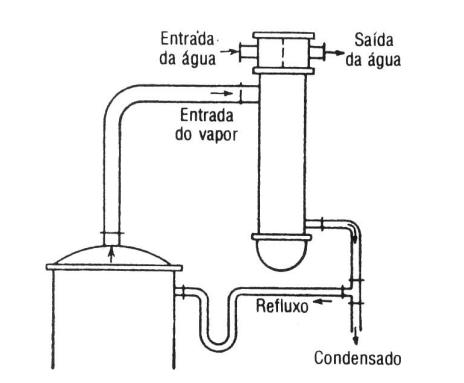
\includegraphics[scale=0.4]{editaveis/figuras/condensador}
	  \caption[Condensador]{Condensador\footnotemark}
	  \label{condensador}
	\end{figure}	   
	\footnotetext{Disponível em: http://www.essel.com.br/cursos/material/03/Ap12.pdf}
	\FloatBarrier
	\begin{figure}[!htbp]
	 \centering
	  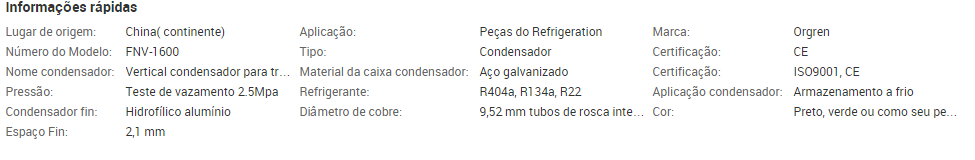
\includegraphics[scale=0.4]{editaveis/figuras/informacao_condensador}
	  \caption[Informações sobre o condensador]{Informações sobre o condensador\footnotemark}
	  \label{condensador_informacao_1}
	\end{figure}	
	\footnotetext{Disponível em:http://portuguese.alibaba.com/product-gs/vertical-condenser-for-heat-exchange-60225996798.html}   
	\FloatBarrier	
	\begin{figure}[!htbp]
	 \centering
	  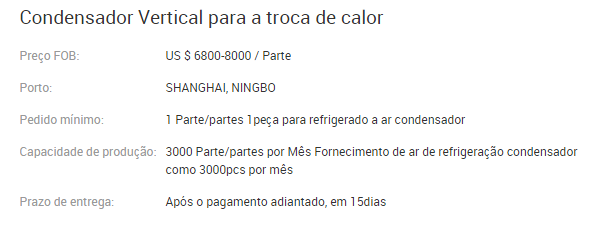
\includegraphics[scale=0.4]{editaveis/figuras/condensador_vertical}
	  \caption[Informações sobre o condensador 2]{Informações sobre o condensador\footnotemark}
	  \label{condensador_informacao_2}
	  \footnotetext{Disponível em: http://portuguese.alibaba.com/product-gs/vertical-condenser-for-heat-exchange-60225996798.html }
	\end{figure}
		\FloatBarrier